\chapter{Evaluierung}

\section{Test}
Die Verifikation der DSL und ihrer Komponenten wird auf zwei Arten durchgeführt: Zum einen mit automatisierten Modultests und zum anderen mit manuellen Integrationstests. Erstere zielen darauf ab die Funktionsweise von Editor, Transformator und Validierer einzeln zu testen, um zu verifizieren dass diese ihre Anforderungen erfüllen. Letztere sollen das Zusammenspiel aller Module der DSL prüfen indem der Erstellungsprozess für verschiedene Konversationsroutings von der Modellierung bis zur Ausführung des Routings nachvollzogen wird.

\subsection{Automatisierte Tests}
Für die automatisierten Tests der DSL-Komponenten kommen Modultests, auch Unit Tests genannt, zum Einstaz. Befürworter der Unit Testing-Praktik befürworten an dieser Technik unter anderem eine hohe Testabdeckung und die frühe Detektierung von Fehlerzuständen [CITATION]. In der vorliegenden Ausarbeitung wird das Unit Test-Verfahren mit Hilfe des .NET-Test-Frameworks XUnit umgesetzt. Dabei werden Methoden mit einem Attribut als Test-Methoden designiert, welche dann von XUnit ausgeführt und ausgewertet werden. Die Testmethoden folgen dem Arrange-Act-Assert-Entwicklungsmuster. Hierbei ist eine Methode in drei Phasen aufgeteilt: In der Arrange-Phase werden die für den Test nötigen Vorbereitungen wir Objekt-Initialisierungen etc. durchgeführt. Anschließend folgt die Act-Phase, in der die zu testende Aktion durchgeführt wird. In der Assert-Phase wird das Testergebnis mit Assertions überprüft. Schlägt keine der Assertions fehl, gilt ein Testfall als bestanden.

\subsubsection{Editor}
In der Editor-Komponente werden zwei Klassen getestet: FlowDiagramViewModel und FlowDiagramControl. Die beiden Komponenten sind vor allem über die Datenbindung des Devexpress-Frameworks miteinander verbunden. Da das Testen dieser Verbindung jedoch außerhalb des Zuständigkeitsbereichs für die vorliegende Ausarbeitung ist, werden die beiden Klassen unabhängig voneinander getestet. Für FlowDiagramViewModel ist besonders das Verhalten bei Veränderungen in der Model-Schicht interessant, vor allem wenn es um das Hinzufügen oder Entfernen von Verbindungen geht. Folgende Aspekte der Klasse FlowDiagramViewModel werden unter anderem in den vorliegenden Unit Tests verfiziert: 

\begin{itemize}
\item Das Speichern von Flow-Instanzen im Dateisystem funktioniert
\item Das Laden von Flow-Instanzen aus dem Dateisystem funktioniert
\item Beim Hinzufügen von Connector-Instanzen werden die zugehörigen Input-Referenzen in betroffenen Outputs korrekt gesetzt
\item Beim Entfernen von Connector-Instanzen werden die zugehörigen Input-Referenzen in betroffenen Outputs auf null gesetzt
\item Beim Setzen einer Input-Referenz in einem Output wird eine entsprechende Connector-Instanz hinzugefügt
\item Beim Setzen einer Input-Referenz auf null in einem Output wird die entsprechende Connector-Instanz entfernt
\item Beim Verändern einer Input-Referenz in einem Output auf eine andere Input-Instanz wird der entsprechende Connector aktualisiert 
\end{itemize}

Auch bei der Klasse FlowDiagramControl fokussieren sich die Testfälle auf das Verhalten im Fall einer Veränderung der Daten, die per Datenbindung zur Verfügung stehen. Die Hauptaufgabe von FlowDiagramControl ist es, diese Daten auf Instanzen der Klasse FlowDiagramItem abzubilden. Da die eigentlich Darstellung der FlowDiagramItem-Instanzen von der Basisklasse und damit vom Devexpress-Framework überommen wird, wird dies nicht getestet. Stattdessen prüfen die Testfälle, ob es für jede Connector- und jede Node-Instanz eine entsprechende DiagramItem-Instanz gibt. Die Testfälle verifizieren daher folgende Anforderungen:

\begin{itemize}
\item Das Hinzufügen einer Node-Instanz fügt dem Diagramm eine entsprechende Flow\-Diagram\-Item-In\-stanz hinzu
\item Das Entfernen einer Node-Instanz entfernt auch die entsprechende Flow\-Diagram\-Item-In\-stanz
\item Das Hinzufügen einer FlowDiagramItem-Instanz fügt eine entsprechende Node-Instanz hinzu
\item Das Entfernen einer FlowDIagramItem-Instanz entfernt eine entsprechende Node-Instanz
\item Das Hinzufügen einer Connector-Instanz fügt dem Diagramm eine entsprechende Flow\-Dia\-gram\-Con\-nec\-tor-In\-stanz hinzu
\item Das Entfernen einer Connector-Instanz entfernt auch die entsprechende Flow\-Dia\-gram\-Con\-nec\-tor-In\-stanz
\item Das Hinzufügen einer FlowDiagramConnector-Instanz fügt auch eine entsprechende Connector-Instanz hinzu
\item Das Entfernen einer FlowDiagramConnector-Instanz entfernt auch die entsprechende Connector-Instanz
\item Das Ändern der Endpunkte einer FlowDiagramConnector-Instanz passt auch die entsprechende Connector-Instanz an
\end{itemize} 

\subsubsection{Transformator}  
In den Tests für die Transformator-Komponenten werden die wichtigsten Klassen für die Bytecode-Generierung verifiziert. Dabei ist der Zuständigkeitsbereich einer Klasse zu beachten, und dementsprechend zu testen. Es macht zum Beispiel wenig Sinn, die Details der Syntax der generierten Klassen in den Testfällen für ConversationRoutingBehaviorGenerator zu verifizieren, da sich diese Klasse mit der Kompilierung der Syntax und Erstellung des Bytecodes beschäftigt. Die Syntax der generierten Klassen wird in den Modulen FlowClassSyntaxBuilder und UserCodeClassSyntaxBuilder erstellt und sollte dementsprechend in den dort zugehörigen Testfällen verifiziert werden. Auf diese Weise wird eine unnötige mehrfache Testüberdeckung vermieden. Vor diesem Hintergrund werden für die Klasse ConversationRoutingBehaviorGenerator folgende Aspekte mittels Unit Tests getestet: 

\begin{itemize}
\item Im Falle einer übergebenen korrekten Flow-Instanz wird in der Methode die CIL-Syntax erfolgreich erstellt, kompiliert und ein In-Memory-Assembly wird zurückgegeben, in der die erwartete Konversationsrouting-Klasse definiert ist
\item Im Falle einer übergebenen Flow-Instanz, in der keine Start-Instruktion vorhanden ist, wird eine Exception geworfen
\item Im Falle einer fehlgeschlagenen Kompilierung der generierten Syntax wird eine Exception geworfen, in der detaillierte Fehlermeldungen enthalten sind
\item Im Falle einer korrekten Flow-Instanz wird von Roslyn ein semantisches Modell der CIL-Syntax generiert
\end{itemize} 

Die nächst niedrigere Stufe bei der Transformation ist die Erstellung des CIL-Syntaxbaums. Hierfür wird die Klasse ConversationRoutingSyntaxTreeBuilder folgendermaßen getestet:

\begin{itemize}
\item Im Falle einer übergebenen Start-Instruktion wird erfolgreich ein CIL-Syntaxbaum generiert, welcher auf der höchsten Ebene die Syntax für die erwartete Klassendeklarationen im erwarteten Namespace enthält
\item Im Falle von ungenügenden übergebenen Parametern wird eine Exception geworfen
\end{itemize}

Der Syntaxbaum besteht zum größten Teil aus der Klassendeklaration der Klasse, welche das Konversationsrouting umsetzt. Die Syntax dieser Klasse wird von FlowClassSyntaxBuilder erstellt und im Zuge der zugehörigen Testfälle für diese Klasse verifiziert:

\begin{itemize}
\item Im Falle einer übergebenen Start-Instruktion eines korrekten DSL-Modells wird die Syntax für eine Klasse zurückgegeben, die von ACDCallRoutingBehaviorBase erbt, und für jede im Modell enthaltene Instruktion eine Membermethode beinhaltet. Zusätzlich existiert eine geschachtelte private Klassendeklaration für den benutzerspezifischen Code, welche als Instanz als Membervariable in der umfassenden Klasse vertreten ist
\item Im Falle von fehlerhaften übergebenen Parametern wird eine Exception geworfen.
\end{itemize}

UserCodeClassSyntaxBuilder, welche für die Generierung der geschachtelten Klassendeklaration zuständig ist, wird auf folgende Anforderungen getestet:

\begin{itemize}
\item Im Falle einer übergebenen Start-Instruktion eines korrekten DSL-Modells wird die Syntax für eine Klasse zurückgegeben, in der alle Instruktionen des Modells, die benutzerspezifischen Code enthalten, mit einer Membermethode vertreten sind, die diesen Code ausführt. Zusätzlich existieren für benutzerdefinierte  Funktionen entsprechende Membermethoden und für benutzerdefinierte Variablen entsprechende Membervariablen. Die Klasse enthält weiterhin zwei Properties vom Typ String mit den Namen Skill und Language.
\item Im Falle von fehlerhaften übergebenen Parametern wird eine Exception geworfen.
\end{itemize}

Ob die Syntax für generierte Methoden, die den Ablauf des Routings steuern, die richtige Struktur aufweist, wird in den Testfällen für die Klasse MethodFlowSyntaxBuilder wie folgt getestet:

\begin{itemize}
\item Wird eine Instruktion in Form einer Node-Instanz übergeben, wird eine Liste an Methodendeklarationen zusammengestellt, in der alle von der übergebenen Node erreichbaren Instruktionen abgebildet sind. In der Syntax für jeden Methodenkörper existieren die Methodenaufrufe für die im Modell jeweils nachfolgende Instruktion.
\item Werden unzureichende Parameter übergeben, wird eine Exception geworfen
\end{itemize}

Die Methoden-Deklarationen für die Usercode-Klasse werden von UserCodeMethodSyntaxBuilder umgesetzt und folgendermaßen getestet:

\begin{itemize}
\item Wird eine Instruktion in Form einer Node-Instanz übergeben, wird eine Liste an Methodendeklarationen zusammengestellt, in der nur die Instruktionen abgebildet sind, in denen vom Benutzer geschriebener Code zum Einsatz kommt.
\item Werden unzureichende Parameter übergeben, wird eine Exception geworfen
\end{itemize}

Zuletzt wird noch getestet, ob der Inhalt der generierten Methoden den Anforderungen entspricht. Dafür werden alle von NodeSyntaxBuilder abgeleiteten Typen getestet, da diese die instruktionsspezifische Syntax  für eine Methode generieren:

\begin{itemize}
\item Jeder Subtyp von NodeSyntaxBuilder erstellt für die ihm übergebene Instanz des zugehörigen Node-Subtyps die spezifische Syntax, die notwendig ist, um diese Instruktion umzusetzen. Die Syntax wird in Form einer Liste von SyntaxNode-Instanzen zurückgeliefert 
\item Werden unzureichende Parameter übergeben, wie zum Beispiel eine Instanz eines falschen Node-Subtyps, wird eine Exception geworfen
\end{itemize}

Bei allen Tests, die als Parameter eine Flow-Instanz entgegennehmen, wird das Modell aus Abb. \ref{fig:TestRouting} verwendet. 

\subsection{Manuelle Tests}
Bei den manuellen Tests geht es darum, das korrekte Zusammenwirken der einzelnen Komponenten zu testen. Daher werden alle Schritte, die für die Inbetriebnahme eines Konversationsroutings von Nöten sind, ausgeführt und die korrekte Funktionsweise anschließend verifiziert. Zu diesem Zweck werden folgende Schritte in der beschriebenen Reihenfolge ausgeführt:
\begin{description}
\item[Modellierung] \hfill \\
Hier wird mittels des Editors ein Modell angefertigt und abgespeichert. In dem Modell sind alle Arten von Instruktionen enthalten, welche auch alle mindestens einmal über einen Pfad des Konversationsroutings ausgeführt werden. Das Routing muss mindestens einen Zyklus in seinem Ablauf vorweisen. Zusätzlich sind mindestens je eine benutzerdefinierte Variable und Funktion im Routing enthalten, die auch in einer oder mehreren Script-Instruktionen verwendet werden. Bei der Modellierung des Routings müssen alle Editoren (Script-, Listen-, Ausdrucks- und Routing-Editor) mindestens einmal ausgeführt werden. Nach dem Editieren eines jeden Wertes muss durch erneutes Editieren überprüft werden, ob der Wert auch tatsächlich übernommen wurde. Treten während des Modellierens keine Fehler auf, wird das Routing im Dateisystem abgespeichert. 
\item[Ausführung] \hfill \\
Als nächstes wird die Routing Engine gestartet. Diese ist so konfiguriert, dass sie beim Start das im vorherigen Schritt modellierte Routing lädt und bei einem eingehenden Anruf ausführt.
\item[Anruf] \hfill \\
Nachdem die Routing Engine gestartet ist, kann das Modell über Anrufe getestet werden. Es werden so viele Anrufe getätigt, dass jeder Pfad des Routings einmal ausgeführt wurde und sich das Verhalten mit der Spezifikation des Modells deckt. Insbesondere wird stichprobenartig für jeden Pfad getestet, wie sich das System verhält wenn entweder der Anrufer oder ein beteiligter Agent frühzeitig den Anruf beendet. In diesen Fällen dürfen für ein Bestehen des Tests keine Anrufe auf Agenten- oder Kundenseite mehr übrig bleiben.
\end{description}
Ein Kandidat für ein Test-Routing mit dem die oben stehenden Schritte ausgeführt werden, ist in Abbildung \ref{fig:TestRouting} zu sehen. Neben dem Kriterium, alle Instruktionen zu beinhalten, bietet es eine überschaubare Anzahl an Pfaden die durch das Routing  führen. Dank der frühen DTMF-Instruktion kann zwischen drei Haupt-Pfaden gewählt werden. Werden die beiden Einstiegspunkte mit berechnet, genügen zur vollständigen  Abdeckung dieser Hauptpfade also acht Anrufe. Auf der Abbildung sind die Scripte sowie benutzerdefinierten Variablen und Funktionen, die zum Einsatz kommen, nicht zu sehen. Angelegt ist die Integer-Variable Count, welche im Set Variables-Knoten mit 0 initialisiert wird. Anschließend wird in der Branch-Instruktion abgefragt, ob Count größer als zehn ist und ob es sich um eine gerade Zahl handelt. Letzteres wird mit einer benutzerdefinierten Funktion IsEven überprüft. Die Branch-Instruktion nimmt also zu erst den False-Ausgang, welcher in das erste Script führt. Das Script dort inkrementiert diet Count-Variable um eins und führt zurück in die Branch-Instruktion. Diese Schleife wird solange ausgeführt, bis die Branch-Instruktion den True-Ausgang nimmt. Dieser führt das zweite Script aus, in der die benutzerdefinierte Funktion PrintTime aufgerufen wird, welche die aktuelle Systemzeit auf der Konsole ausgibt.

\begin{figure} %[hbtp]
	\centering
		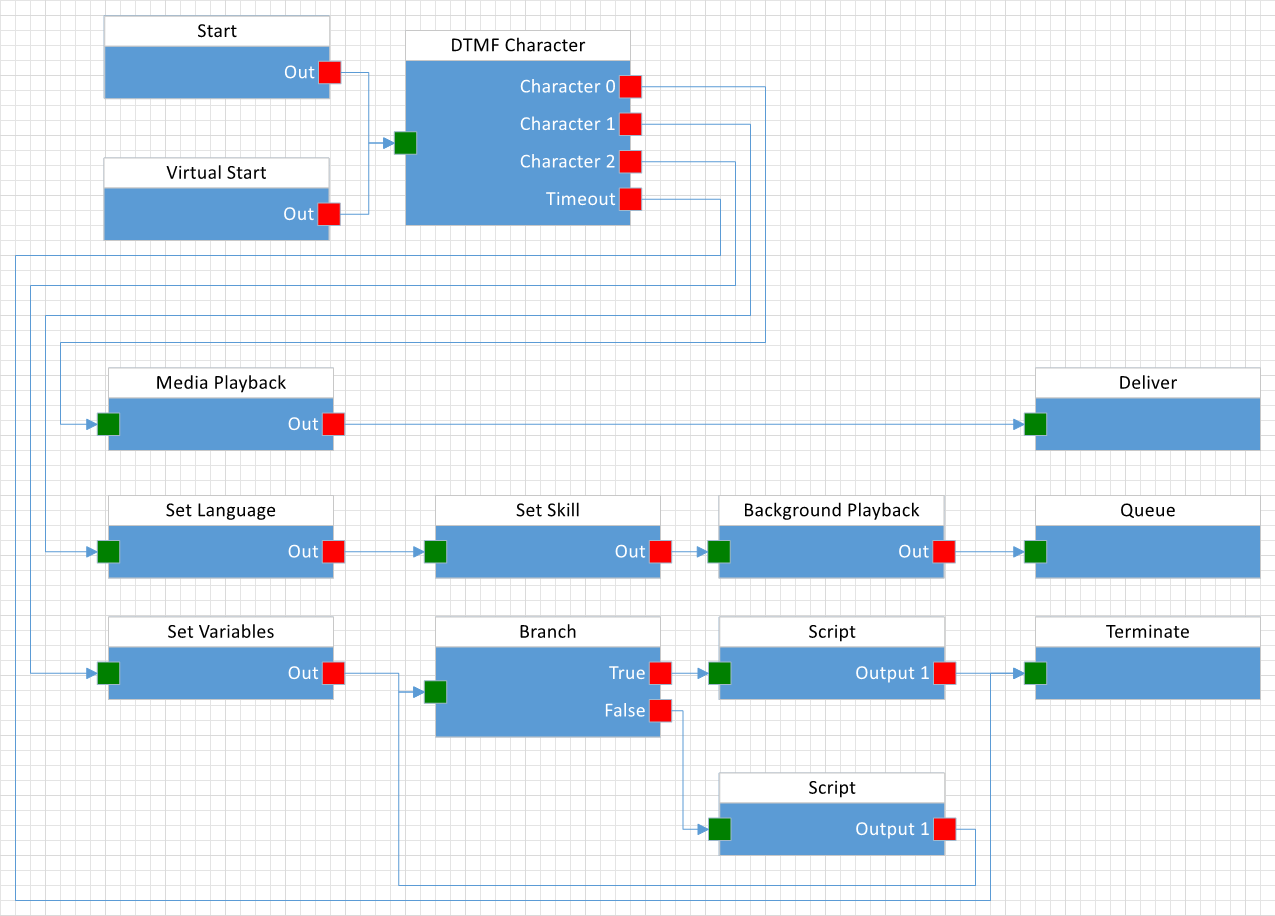
\includegraphics[width=\textwidth]{img/TestRouting.png}
	\caption[DSL-Modell für manuelle Tests]{Zu sehen ist das DSL-Modell, welches im Zuge von automatisierten und manuellen  Tests zum Einsatz kommt.}
	\label{fig:TestRouting}
\end{figure}

\section{Metriken}
Bei der Umsetzung der DSL entstehen zwei Arten von Code. Die eine Art von Quellcode setzt das System um: Es handelt sich hierbei um den Quellcode, der den Editor, den Transformator und die Modell-Validierung implementiert. Die andere Art von Code ist der vom System generierte Code, also der CIL-Bytecode, der ein einzelnes Routing umsetzt. Die erste Code-Art ist für den weiteren Lebenszyklus der DSL von unmittelbarer Bedeutung und muss daher vor allem wartbar sein. Da her folgt eine Einschätzung zur vermessenen Umfang und Komplexität. Diese Vermessungen für die andere Art von Code durchzuführen, wäre  wenig aussagekräftig, da sowohl Umfang als auch Komplexität stark vom transformierten Modell abhängt: Je komplexer und umfangreicher das Konversationsrouting, desto komplexer ist der Code, der dieses Konversationsrouting umsetzt. Die Grenzen sind vor allem nach oben nicht abschätzbar, da der Benutzer in Script-Instruktionen und eigenen Funktionen ``unvorhersehbaren'' Code einfügen kann. Da außerdem aus der erstellten Syntax für Benutzer unleserlicher Bytecode generiert wird, welcher nicht dafür gedacht ist per Hand gewartet zu werden, ist das Berechnen von detaillierten Metriken für den so erstellten Code wenig zielführend. 

\subsection{Geschriebener Code}
Berechnet wurden die folgenden Metriken mit der Entwicklungsumgebung Visual Studio 2017 Ultimate. Zum Einsatz kommen die ``Executable Lines of Code'', um einen generellen Überblick über den Umfang der Code-Basis zu liefern, und die zyklomatische Komplexität, auch als McCabe-Metrik bekannt, welche den Grad an Verzweigungnen im Programmfluss beschreibt. Beide Metriken sind im Feld der Software-Architektur verbreitete Maße, deren Berechnung unter anderem in [CITATION] nachgelesen werden kann. Da die Angaben für gesamte Namespaces gemacht werden, wird bei der zyklomatischen Komplexität der Mittelwert und der Median über alle Methoden dieses Namespaces angegeben. Alle der genannten Namespaces sind Unter-Namespaces von ilogixx.ConversationFlow. In Tabelle \ref{tab:metrikenGeschriebenerCode} sind die gemessenen Metriken für den im Zuge der vorliegenden Arbeit händisch verfassten Code zu sehen.
\begin{center}
    \begin{tabular}{| p{0.18\textwidth} | p{0.18\textwidth} | p{0.18\textwidth} | p{0.18\textwidth} | p{0.18\textwidth} |}
    \hline
    Komponente & Namespace & LOC & zykl. Kompl. (mittel) & zykl Kompl. (median)\\ \hline
    Semantisches Modell & Core & 183 & 1,146341463 & 1 \\ \hline
    Editor & UI & 2818 & 2,212669683 & 1 \\ \hline
    Transformator & Generation & 742 & 1,715846995 & 1 \\ \hline
    Validator & Validation & 186 & 1,806451613 & 1 \\ \hline
    \end{tabular}
    \label{tab:metrikenGeschriebenerCode}
\end{center}
Das semantische Modell weist mit der geringsten Anzahl an Lines of Code und der kleinsten durchschnittlichen zyklomatischen Komplexität die niedrigste Komplexität auf. Dies ist nicht überraschend, da es sich um eine fast reine Datenstruktur handelt, die wenig programmatisches Verhalten aufweist. An zweiter Stelle kommt die Komponente der Modell-Validierung. Komplexe Abläufe und ein hoher Umfang an Code, konnte hier vermieden werden, da die meiste Arbeit, welche die Metriken erhöhen könnte, an andere Komponenten ausgelagert wird, wie zum Beispiel den Transformator. Dieser weist eine höhere Verzweigung des Programmablaufs und einen größeren Umfang auf, wie die Metriken zum Ausdruck bringen. Dennoch bleibt auch hier die durchschnittliche McCabe-Metrik deutlich unter dem empfohlenen Wert von zehn, auch dank der rekursiven Vorgehensweise dieser Komponente. Durch diese werden Schleifen vermieden, welche einen hohen Einfluss auf die Anzahl an mögliche Programmpfaden haben. Der hohe Anteil an Lines of Code für den Transformator lässt sich durch den Gebrauch der Roslyn-API begründen, welcher aufgrund des Aufbaus eines kompletten Syntaxbaums ausschweifend ausfällt. 
\newline
Die laut den oben stehenden Metriken komplexeste Komponente der DSL ist der Editor. Der im Vergleich extrem hohe LOC-Wert für diese Komponente lässt sich damit begründen, dass automatisch generierter Code des Devexpress-Framework in diesem Namespace enthalten ist. Devexpress benutzt einen sogenannten Component Designer, welcher "Boilerplate"-Code zum Erstellen von Windows Forms-Komponenten automatisch generiert. Dieser Code ist sehr umfangreich, fällt aber wenig ins Gewicht, da der vom Component Designer generierte Code nicht von Hand lesbar oder editierbar sein soll und damit nicht die Komplexität des System widerspiegelt. Der Mittelwert der zyklomatischen Komplexität ist auf die Fallunterscheidungen zurückzuführen, die auf View- und ViewModel-Ebene durchgeführt werden, wenn es um die Behandlung von Events geht, welche durch die Benutzung der grafischen Benutzeroberfläche ausgelöst werden.
\newline
Erwähnenswert ist weiterhin, dass keine Komponente beim Median der zyklomatischen Komplexität den Wert eins überschreitet. In Verbindung mit dem geringen Mittelwert alle Komponenten spricht dies für eine hohe Gradlinigkeit während des Programmablaufs. 

\section{Performanz}
Sowohl der generierte als auch der händisch verfasste Code muss eine hohe Leistungsfähigkeit aufweisen. Aber ähnlich wie im vorangegangen Kapitel gestaltet sich die Abschätzung der Performanz für den generierten Bytecode als schwierig: Der Code kann nur so effizient sein, wie der Benutzer ihn gestaltet. Zusätzlich haben Maße wie Zeitmessungen wenig Bedeutung, da ein Konversationsrouting an vielen Stellen gewünschter Maßen blockiert. Eine Laufzeitanalyse ist in diesem Fall ebenfalls wenig zielführend, da die Laufzeit des Algorithmus, der ein Konversationsroutings ausführt, von keiner Eingabe abhängig ist, sondern höchstens von der Interaktion mit einem Anrufer.
\newline
Aus diesem Grund konzentriert sich die folgende Analyse auf den Code, welcher die Transformation durchführt. Auch hier ist eine hohe Performanz wichtig, da dieser Code im Zuge der Modell-Validierung und damit laufend während der Modellierung ausgeführt wird. Leistungsfähiger Code kann hier also dafür sorgen, dass der Benutzer schnelles Feedback über etwaige Fehler bekommt und bei der Modellierung nicht lange auf die Transformation warten muss.

\subsection{Geschriebener Code}

\subsubsection{Abschätzung der Komplexität}
Bei der Transformation eines DSL-Modells wird dieses wie ein Graph aufgefasst und entsprechend einer Depth-First-Vorgehensweise traversiert. Sei ein Graph definiert als $G = (V, E)$ mit $V$ als der Menge an Knoten und $E \subseteq V^{2}$ als die Menge an Kanten. Die Komplexität eines Depth-First-Algortihmus befindet sich dann in der Komplexitätsklasse $O(\left\vert{V}\right\vert + \left\vert{E}\right\vert)$ (siehe [CITATION]). Bei der Interpretation eines DSL-Modells als Graph werden alle Input-, Node- und Output-Instanzen wie die Knoten, und alle Referenzen zwischen diesen Instanzen wie die Kanten eines Graphen behandelt. Sei daher $V_{dsl}$ die Menge aller dieser Instanzen und $E_{dsl}$ die Menge aller Referenzen zwischen diesen Instanzen. Seien weiterhin $Var$ und $Fun$  je die Mengen aller benutzerdefinierten Variablen und Funktionen. Der Aufwand zur Erstellung der Syntax für eine Instruktion wird als konstant angenommen, da dieser nicht von der Eingabe abhängt. Dabei handelt es sich wohlgemerkt um eine Vereinfachung des Sachverhalts, da der Aufwand, den die Roslyn API betreibt, nicht an allen Stellen zuverlässig abgeschätzt werden kann. 
\newline
Unter den oben genannten Voraussetzungen lässt sich der Aufwand für die Transformation eines DSL-Modells zu einer CIL-Syntax abschätzen als:
$$ O( \left\vert{V_{dsl}}\right\vert + \left\vert{E_{dsl}}\right\vert + \left\vert{Var}\right\vert + \left\vert{Fun}\right\vert ) $$
Die Summierung der Kardinaltiäten von $V_{dsl}$ und $E_{dsl}$ ergibt sich aus der Traversierung des DSL-Modells. Die beiden Summanden $\left\vert{Var}\right\vert$ und $\left\vert{Fun}\right\vert$ ergeben sich aus der Generierung der zugehörigen Syntax, für die durch diese Mengen iteriert werden muss. Außerdem sei angemerkt, dass die Traversierung des DSL-Modells für eine einzelne Transformation dreimal stattfinden muss (Zweimal für je zwei Klassendeklarationen und einmal zur Sammlung aller asynchronen Instruktionen, vergleiche Abs. \ref{subsubsec:Nebenlaeufigkeit}. Da es sich jedoch um einen konstanten Multiplikator handelt, kann dieser weggelassen werden (siehe [CITATION]). 

\subsubsection{Zeitmessungen}
TODO